\documentclass{csnotes}
\usepackage{xcolor}
\usepackage[italian]{babel}
\usepackage{geometry}
\usepackage{graphicx}
\usepackage{xcolor}
\usepackage{hyperref}
\usepackage{listings}
\usepackage{xcolor}
\usepackage{listings}
\usepackage{forest}

\definecolor{tableborder}{rgb}{0.85,0.85,0.85}


% Define custom colors
\definecolor{codegray}{rgb}{0.5,0.5,0.5}
\definecolor{codebg}{rgb}{0.96,0.96,0.96}
\definecolor{keywordcolor}{rgb}{0.0,0.2,0.6}
\definecolor{stringcolor}{rgb}{0.8,0.1,0.1}

\lstdefinelanguage{turtle}{
  morekeywords={@prefix, @base},
  morecomment=[l]{\#},
  morestring=[b]",
  sensitive=true
}

\lstset{
  language=turtle,
  basicstyle=\small\ttfamily,
  keywordstyle=\color{purple}\bfseries,
  stringstyle=\color{teal},
  commentstyle=\color{gray}\itshape,
  numbers=none,
  frame=single,
  rulecolor=\color{lightgray},
  backgroundcolor=\color{gray!5},
  breaklines=true,
  tabsize=2,
  showstringspaces=false
}
\geometry{
    top=2cm,
    bottom=2cm,
    left=2cm,
    right=2cm
}
% Define SPARQL language styling for listings
\lstdefinelanguage{SPARQL}{
  morekeywords={PREFIX, SELECT, WHERE},
  sensitive=true,
  morecomment=[l]{\#},
  morestring=[b]",
  morestring=[b]'
}

\lstset{
  language=SPARQL,
  backgroundcolor=\color{codebg},
  basicstyle=\ttfamily\small,
  keywordstyle=\bfseries\color{keywordcolor},
  commentstyle=\color{codegray},
  stringstyle=\color{stringcolor},
  numbers=left,
  numberstyle=\tiny\color{codegray},
  stepnumber=1,
  numbersep=10pt,
  showstringspaces=false,
  breaklines=true,
  frame=single,
  rulecolor=\color{black!20},
  tabsize=2,
  captionpos=b
}
% Document meta
\title{Intelligent Web}
\author{Giuliano Savino}
\date{\today}

% Title page info
\university{Università Degli Studi Di Napoli Federico II}
\department{Dipartimento Di Ingegneria Elettrica \\ e Delle Tecnologie Dell'Informazione}
\course{Corso Di Laurea Magistrale In Informatica}
\subject{Intelligent Web}
\academicyear{Academic Year 2026/2027}

\begin{document}
\thispagestyle{empty}
\begin{flushright}
    \small
    \textbf{Intelligent Web}\\
    \textit{Scritto da : Giuliano Savino}
\end{flushright}

\vspace{-0.15cm}
\noindent
\textcolor{blue!60!black}{\rule{\textwidth}{1.2pt}}
\vfill
\begin{center}

    {\Large \textbf{Intelligent Web}}\\[0.2cm]
        
    {\large \textit{Scritto da : Giuliano Savino}}

\end{center}

\vfill

\tableofcontents
\newpage
\chapter{RDF}

\begin{definition}{RDF}

    RDF (Resource Description Framework) è uno standard per rappresentare
    informazioni e relazioni tra risorse attraverso triple:

    \begin{center}
        $(soggetto, predicato, oggetto)$
    \end{center}

    Ogni tripla è detta \textbf{statement}.

\end{definition}

Dove:

\begin{itemize}

    \item \textbf{Soggetto}: è la risorsa di cui si parla
    nell'informazione.

    \item \textbf{Predicato}: rappresenta una proprietà o una relazione
    tra il soggetto e l'oggetto.

    \item \textbf{Oggetto}: è la risorsa o il valore a cui si riferisce
    la proprietà.

\end{itemize}

In RDF si introducono due concetti importanti: quello di URI e quello
di risorsa.

\begin{definition}{URI}

    Un URI è una stringa che identifica una risorsa.

\end{definition}

\begin{definition}{Risorsa}

    Una risorsa è qualsiasi entità che può essere identificata e descritta
    mediante un identificatore, come un URI.

    Può rappresentare, ad esempio:

    \begin{itemize}
        \item una cosa del mondo reale;
        \item una proprietà o una relazione;
        \item un'entità astratta.
    \end{itemize}

\end{definition}

\begin{center}
    L'idea di base di RDF è quella di identificare e descrivere le risorse
    mediante opportuni identificatori, in particolare URI/IRI.
\end{center}

\begin{observation}{Grafo RDF}

    L'insieme delle triple RDF può essere rappresentato come un
    \textbf{grafo diretto etichettato}: le risorse rappresentano i nodi,
    mentre i predicati rappresentano gli archi, orientati dal soggetto
    verso l'oggetto.

    Questo permette di concatenare più triple, utilizzando l'oggetto
    di una tripla come soggetto di un'altra.

\end{observation}
\newpage


Quindi a questo punto, soggetto predicato e oggetto, sono tutte delle risorse, cioè \textbf{degli URI}.


Il fatto è che io vorrei anche non avere solo risorse in RDF, ma vorrei esprimere anche \textbf{Interi,Booleani,Stringhe\dots}


A questo ci servono i Literal:

\section{Literal}

\begin{definition}{Literal}
    Un literal rappresenta un valore concreto, come:
    \begin{itemize}
        \item "Diego Maradona"
        \item "Argentina"
        \item  123
        \item 30-10-1960
    \end{itemize}
\end{definition}
\begin{warning}{Literal $\neq$ Risorsa}
Un literal non è una risorsa, una risorsa è una qualunque cosa identificabile tramite un URI.
\end{warning}

I litterali possono essere di due tipi:
\begin{itemize}
    \item tipati.
    \item non tipati.
\end{itemize}
\begin{figure}[htbp]
    \centering
    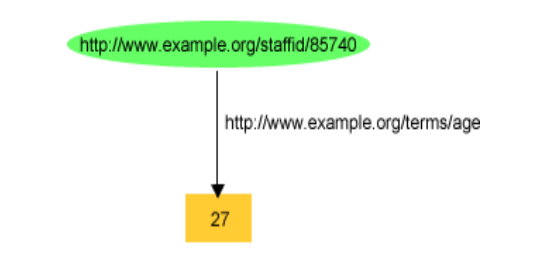
\includegraphics[width=0.7\textwidth]{_files/_images/rdf1.png}
    \caption{Risorsa collegata ad un Literal Non tipato}
    \label{fig:etichetta}
\end{figure}
In questo caso, 27 è non tipato, perchè non stiamo specificando il suo tipo.

\newpage    

\begin{definition}{Letterale Tipato}
    Un litterale tipato è formato da una stringa,e un URI, \textbf{che ne specifica il tipo}.

    La sintassi è la seguente:
    \begin{center}
        \texttt{stringa\string^\string^URIref}
    \end{center}
    dove URIref, è l'uri del datatype, del valore nella stringa, che ne specifica il tipo.
\end{definition}

\begin{example}{Esempio di letterale tipato}
    \texttt{"27"\string^\string^http://www.w3.org/2001/XMLSchema\#integer}
\end{example}

RDF non definisce un insieme di datatype, esistono definiti quindi esternamente a RDF, tipicamente, RDF prende i datatype da XML Schema.


Il datatype, è formato da 3 parti principali:
\begin{itemize}
    \item \textbf{Value Space} : È l'insieme dei valori effettivi che appartengono a quel tipo.
    Per xsd::integer è
    \begin{lstlisting}
        ..., -2, -1, 0, 1, 2, 3, ..., 42, ... 
    \end{lstlisting}
    questi rappresentano i valori di quel tipo
    \item \textbf{Lexical space}
    È l'insieme delle stringhe ammesse per rappresentare quei valori.
    Per esempio, per il valore 42, si ha:
    \begin{itemize}
        \item "42"
        \item "+42"
    \end{itemize}
    \item \textbf{Lexical-to-value mapping} : Questa è semplicemente la funzione che dice:
    \begin{center}
        "Questa stringa, quale valore rappresenta?"
    \end{center}
    Quindi collega, il valuespace al lexical space, è il ponte fra i due spazi.
    Per esempio:
    \begin{lstlisting}
        "42"  --------->  42
        "+42" --------->  42
    \end{lstlisting}
\end{itemize}
\begin{center}
    \textbf{I literal, possono comparire solo come oggetti.Quindi nella tripla, sono comparire solo come terzo elemento}
\end{center}
Quindi facendo il punto della situazione,per ora con RDF possiamo rappresentare, risorse (che sono identificate da un URI) e letterali.


Le triple per ora, saranno qualcosa del genere:
\begin{example}{Esempio Triple in RDF}

Consideriamo la seguente informazione:

\begin{center}
\textbf{Diego Maradona ha come data di nascita il 30-10-1960.}
\end{center}

Possiamo rappresentarla tramite la seguente tripla RDF:

\begin{center}
\texttt{(Maradona, dataDiNascita, "30-10-1960")}
\end{center}

dove:

\begin{itemize}
\item \texttt{Maradona} è il \textbf{soggetto}, cioè una risorsa identificata tramite un URI;
\item \texttt{dataDiNascita} è il \textbf{predicato}, anch'esso identificato tramite un URI;
\item \texttt{"30-10-1960"} è l'\textbf{oggetto}, che in questo caso è un literal, non tipato, e quindi lo si interpreta come una stringa.
\end{itemize}

Quindi una tripla RDF può avere come oggetto sia una \textbf{risorsa} sia un \textbf{literal}.

Ad esempio:

\begin{center}
\texttt{(Maradona, giocaPer, SSC Napoli)}
\end{center}

ha come oggetto una \textbf{risorsa}, mentre:

\begin{center}
\texttt{(Maradona, numeroMaglia, "10"\string^\string^\texttt{http://www.w3.org/2001/XMLSchema\#integer})}
\end{center}

ha come oggetto un \textbf{literal tipato}.
\end{example}

\begin{center}
Quindi in RDF, per ora, le triple sono formate da URI (soggetto, predicato, oggetto) e,limitatamente alla posizione di oggetto, da letterali.    
\end{center}

\begin{definition}{Modello dei Dati RDF}
    RDF (parliamo di RDF base senza serializzazioni, quindi come modello dei dati) definisce un modello di dati astratto basato su un insieme di triple:
    \begin{center}
        (s,p,o)
    \end{center}
    Dove:
    \begin{itemize}
        \item \textbf{s} = soggetto.
        \item \textbf{p} = predicato.
        \item \textbf{o} = oggetto.
    \end{itemize}
    Dove il soggetto può essere una risorsa,o un blank node, il predicato deve essere una risorsa, e l'oggetto può essere una risorsa,literal o blank node.
\end{definition}

\section{URI e URL}
L'URI è lo standard generale per denotare qualsiasi risorsa, reale o astratta.
Gli URIs(a differenza degli URL) non si limitano a denotare risorse che sono deferenziabili sul Web,
ovvero che hanno una locazione sulla rete.

\begin{definition}{URL}
    L'URL è una stringa che identifica una risorsa deferenziabile, cioè che interrogandola sul web, mi restituisce qualcosa, \textbf{questo implica}
    che a quella stringa corrisponda un \textbf{meccanismo di accesso (http, ftp, ecc.), che permette di recuperare effettivamente la risorsa in rete}.

    Quindi se prendo un URL e lo "cerco" (cioè lo dereferenzi, ad esempio digitandolo nel browser),
    il sistema sa esattamente dove andare a bussare e — se tutto funziona correttamente — ottieni indietro la risorsa stessa (una pagina HTML, un'immagine, un file...).

    Con l'URI generico questo non è garantito.
\end{definition}


Gli URI possono identificare invece anche risorse non deferenziabili, cioè che \textbf{non ha nessuna locazione di rete associata}, 
ad esempio una persona, un concetto astratto, una proprietà.



RDF usa gli URI, perchè se ne infischia della deferenziabilità, basta identificare le risorse insomma, mentre ad esempio il browser,\textbf{assume}
che io gli stia dando un URL, quindi tenta sempre di dereferenziarlo per restituirti un contenuto, nel caso di alcuni URI, ovviamente questa 
deferenziazione non va a buon fine, per quello detto prima.

\subsection{URI schemes}
Ci sono diversi schemi di URI che sono usati per vari scopi, per identificare risorse in modo differente:
\begin{itemize}
    \item \textbf{http} : HypertextTransfer Protocol, per denotare la locazione di pagine Web. (In questo caso è anche un URL)
    \item \textbf{mailto} : indirizzi email, e.g., mailto:em@w3.org
    \item \textbf{ftp} : FileTransfer Protocol.
\end{itemize}
\section{URIrefs}
\begin{definition}{URIrefs}
    URIrefs = URI + frammento identificativo
\end{definition}
\begin{example}{URIrefs}
    http://www.example.org/index.html\#section2

    \begin{itemize}
        \item è formato da un URI (http://www.example.org/index.html), che è la risorsa, cioè la pagina.
        \item e un frammento identificativo : \#section2 ad esempio una parte specifica dentro quella pagina.
    \end{itemize}
\end{example}
Gli URIrefs possono essere assoluti o relativi.

\begin{example}{URIrefs relativo}
    URIref relativo \#section2 quando occorre nella risorsa http://www.example.org/index.html 
    viene completato ottenendo URIref assoluto http://www.example.org/index.html\#section2
\end{example}

\begin{observation}{URIrefs in HTML vs RDF}
    Una differenza sostanziale fra come gli URIrefs sono usati in HTML e RDF è laseguente. 
    Si consideri per esempio gli URIrefs:
    \begin{itemize}
        \item http://www.example.org/index.html
        \item http://www.example.org/index.html\#Section2
    \end{itemize}
    Nell'uso abituale di HTML, questi URIrefs sono correlati: entrambi si riferiscono allo stesso documento, 
    in particolare il secondo identifica una locazione all'interno del primo.


    RDF invece non fa nessuna particolare assunzione, i due riferimenti sono per RDF
    completamente irrelati. Essendo URIrefsintatticamente differenti possono riferirsi a
    risorse completamente diverse. 
\end{observation}
\section{Serializzazioni}

Finora abbiamo parlato di \textbf{RDF come modello di dati}, ovvero come un insieme di triple della forma

$$
(soggetto,\ predicato,\ oggetto)
$$

dove soggetto, predicato e oggetto possono essere risorse identificate tramite URI, mentre l'oggetto può essere anche un \textbf{literal} o un \textbf{blank node}, mentre il soggetto può essere anche un blank node.

Una serializzazione è una particolare sintassi che permette di trasformare il modello RDF in una rappresentazione testuale o, più in generale, in un formato memorizzabile e scambiabile.

Esistono diverse serializzazioni RDF, tra cui:

\begin{itemize}
\item \textbf{Turtle}: sintassi compatta e leggibile, che permette di utilizzare prefissi e abbreviazioni;
\item \textbf{RDF/XML}: serializzazione di RDF basata sulla sintassi XML;
\item \textbf{JSON-LD}: serializzazione basata su JSON, particolarmente adatta allo scambio di dati sul Web;
\item \textbf{N-Triples}: serializzazione molto semplice, in cui ogni tripla viene rappresentata esplicitamente;
\item \textbf{N-Quads}: estensione di N-Triples che permette di rappresentare anche più grafi RDF.
\end{itemize}

Le diverse serializzazioni \textbf{non definiscono modelli RDF differenti}: rappresentano lo stesso modello di dati attraverso sintassi differenti.

Ad esempio, la stessa informazione RDF

\[
\left(
\texttt{http://example.org/Mario},
\texttt{http://xmlns.com/foaf/0.1/name},
\texttt{"Mario"}
\right)
\]

può essere rappresentata in Turtle come:

\begin{verbatim}
@prefix ex: http://example.org/ .
@prefix foaf: http://xmlns.com/foaf/0.1/ .

ex:Mario foaf:name "Mario" .
\end{verbatim}

oppure in N-Triples come:

\begin{verbatim}
http://example.org/Mario
http://xmlns.com/foaf/0.1/name
"Mario" .
\end{verbatim}

Le due rappresentazioni hanno \textbf{lo stesso significato a livello del modello RDF}; cambia solamente la sintassi utilizzata per serializzarlo.

In particolare, elementi come \textbf{prefissi, QNames e abbreviazioni sintattiche} non fanno parte del modello RDF astratto, ma sono caratteristiche offerte da alcune specifiche serializzazioni. Ad esempio, il QName

$$
\texttt{foaf:name}
$$

è una forma abbreviata utilizzabile in Turtle, ma il modello RDF considera comunque l'URI completo:

$$
\texttt{http://xmlns.com/foaf/0.1/name}.
$$


Il \textbf{modello RDF} definisce la struttura e il significato dei dati, mentre la \textbf{serializzazione} definisce come tali dati vengono concretamente rappresentati e scritti.

\section{Turtle}

Turtle è una sintassi di serializzazione per RDF che permette di rappresentare
le triple RDF in una forma più compatta e leggibile.

\begin{itemize}

    \item Uno statement semplice ha la stessa sintassi della Triple Notation:
    
    \begin{center}
        \texttt{people:Ryan ext:worksWith people:John .}
    \end{center}

    \item Più statement che condividono lo stesso soggetto possono essere
    scritti in forma sintetica, scrivendo il soggetto una sola volta e
    utilizzando il punto e virgola (\texttt{;}) tra i diversi statement.

    \begin{center}
        \texttt{people:Andrew foaf:knows people:Matt ;}\
        \texttt{\phantom{people:Andrew }foaf:surname "Perez-Lopez" .}
    \end{center}

    Questa forma è equivalente a scrivere separatamente:

    \begin{center}
        \texttt{people:Andrew foaf:knows people:Matt .}\
        \texttt{people:Andrew foaf:surname "Perez-Lopez" .}
    \end{center}

    \item Più statement che condividono lo stesso soggetto e predicato
    possono essere raggruppati utilizzando la virgola (\texttt{,}).

    \begin{center}
        \texttt{people:Andrew foaf:knows people:Matt , people:Ryan , people:John .}
    \end{center}

    Questa forma è equivalente alle tre triple:

    \begin{center}
        \texttt{people:Andrew foaf:knows people:Matt .}\
        \texttt{people:Andrew foaf:knows people:Ryan .}\
        \texttt{people:Andrew foaf:knows people:John .}
    \end{center}

\end{itemize}


\subsection{Blank Node}

I blank node possono essere espressi utilizzando dei riferimenti anonimi \texttt{\_:x} oppure attraverso una forma compatta mediante parentesi quadre \texttt{[,]}.

\vspace{1em}

\noindent
\begin{minipage}[t]{0.48\textwidth}
\textbf{Uso di riferimenti anonimi (\texttt{\_:abc}):}
\begin{lstlisting}
@prefix rdf: <http://www.w3.org/1999/02/22-rdf-syntax-ns#>.
@prefix dc: <http://purl.org/dc/elements/1.1/>.
@prefix exterms: <http://www.example.org/terms/>.

<http://www.w3.org/TR/rdf-syntax-grammar>
    dc:title "RDF/XML Syntax Specification (Revised)" ;
    exterms:editor _:abc .

_:abc
    exterms:fullName "Dave Beckett" ;
    exterms:homePage <http://purl.org/net/dajobe/> .
\end{lstlisting}
\end{minipage}
\hfill
\begin{minipage}[t]{0.60\textwidth}
\textbf{Forma compatta con parentesi quadre (\texttt{[]}):}
\begin{lstlisting}
@prefix rdf: <http://www.w3.org/1999/02/22-rdf-syntax-ns#>.
@prefix dc: <http://purl.org/dc/elements/1.1/>.
@prefix exterms: <http://www.example.org/terms/>.

<http://www.w3.org/TR/rdf-syntax-grammar>
    dc:title "RDF/XML Syntax Specification (Revised)" ;
    exterms:editor [
        exterms:fullName "Dave Beckett" ;
        exterms:homePage <http://purl.org/net/dajobe/> .
    ] .
\end{lstlisting}
\captionof{figure}{Qui si va a definire una risorsa <http://www.w3.org/TR/rdf-syntax-grammar>, con un predicato exterms:editor, a cui è collegato un blank node, e a questo blank node ha come nodi uscenti i predicati e risorse che mettiamo dentro}
\end{minipage}


\section{XML}
Un altro tipo di serializzazione molto usata è XML.
Se io voglio rappresentare queste triple di RDF standard:
\begin{figure}[h]
    \centering
    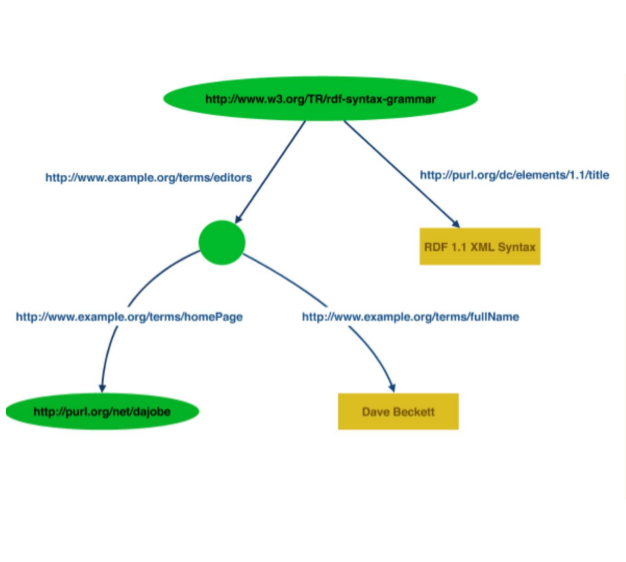
\includegraphics[width=0.5\textwidth]{_files/_images/rdf5.png}
    \caption{RDF abstract syntax}
    \label{fig:etichetta}
\end{figure}
\begin{figure}[h]
    \centering
    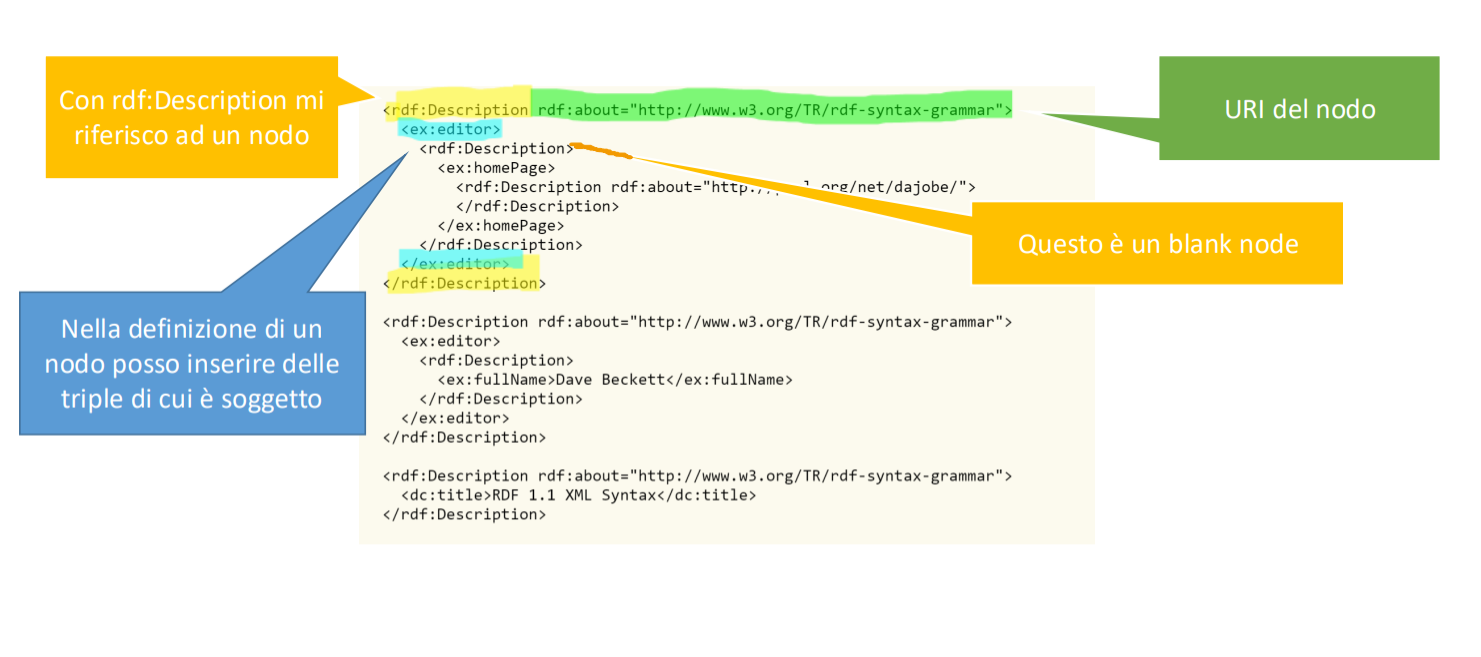
\includegraphics[width=1\textwidth]{_files/_images/rdf6.png}
    \caption{Implementazione nella serializzazione XML (Nota che i literal si rappresentano senza una particolare sintassi)}
    \label{fig:etichetta}
\end{figure}
\begin{figure}[h]
    \centering
    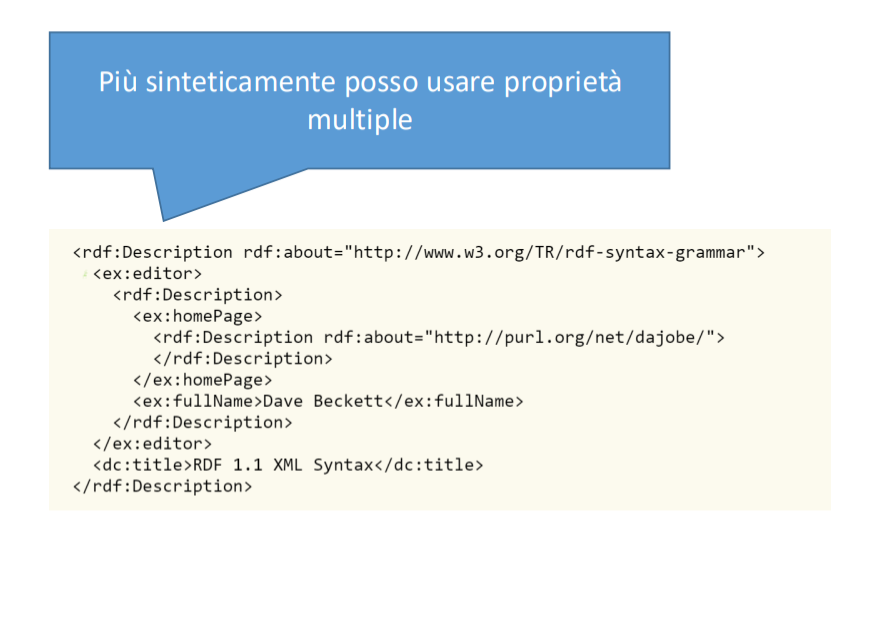
\includegraphics[width=0.6\textwidth]{_files/_images/rdf7.png}
    \caption{Posso immettere altre proprietà, come <dc:title> all'interno dello stesso nodo}
    \label{fig:etichetta}
\end{figure}

\begin{figure}[h]
    \centering
    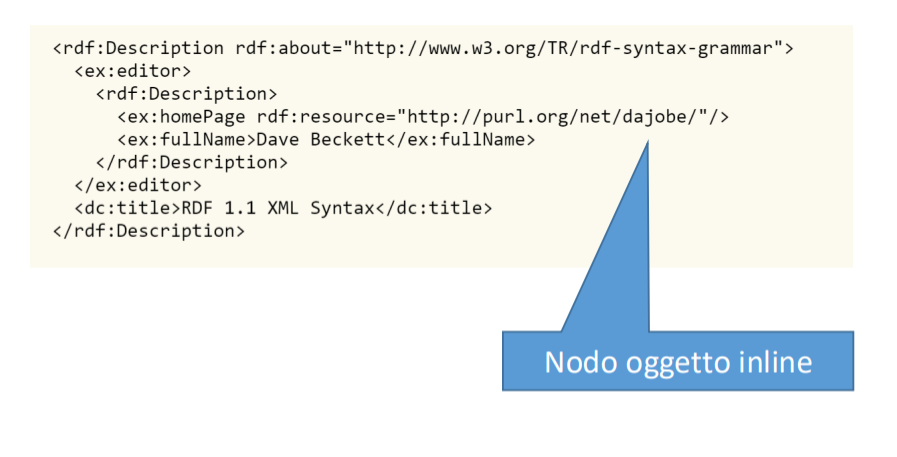
\includegraphics[width=0.6\textwidth]{_files/_images/rdf8.png}
    \caption{Si può usare rdf:resource, per specificare un nodo come oggetto inline}
    \label{fig:etichetta}
\end{figure}

\clearpage

\section{QNames}
I QName non sono elementi del modello RDF, ma una forma sintattica abbreviata per rappresentare gli IRI, 
utilizzata da alcune serializzazioni RDF, come Turtle.

\begin{observation}{RDF abstract syntax}
    RDF, a livello di modello dei dati (il cosiddetto RDF abstract syntax o concrete model), è definito come un insieme di triple:
    \begin{center}
        (soggetto, predicato, oggetto)
    \end{center}
    dove soggetto, predicato e oggetto sono, salvo casi particolari (letterali, blank node), IRI completi. 
    Non esiste, a questo livello, alcun concetto di "prefisso" o abbreviazione — un IRI è un IRI, per intero.
\end{observation}
\begin{example}{QName}
    Un esempio in Turtle:
    \begin{lstlisting}
@prefix ex: <http://example.org/> .
ex:Giuliano ex:age 22 .
    \end{lstlisting}
    Si va a definire un prefisso ex: e ogni volta che si userà davanti ad un nome ad esempio, si appenderà all'URI completo, il nome, in questo modo:
    \begin{center}
        <http://example.org/age>
    \end{center}
\end{example}
Alcune abbreviazioni usate spesso:
\begin{itemize}
    \item \texttt{rdf:} \quad namespaceURI: \url{http://www.w3.org/1999/02/22-rdf-syntax-ns#}
    \item \texttt{dc:} \quad namespaceURI: \url{http://purl.org/dc/elements/1.1/}
    \item \texttt{owl:} \quad namespaceURI: \url{http://www.w3.org/2002/07/owl#}
    \item \texttt{ex:} \quad namespaceURI: \url{http://www.example.org/}
    \item \texttt{xsd:} \quad namespaceURI: \url{http://www.w3.org/2001/XMLSchema#}
\end{itemize}
\section{Vocabolari}
In RDF, per identificare risorse e proprietà si usano degli URI, come abbiamo visto in modo precedente.

\begin{definition}{Vocabolario RDF}
    Un vocabolario RDF è un insieme di termini identificati da URI, 
    generalmente classi e proprietà, utilizzati per descrivere le risorse di uno specifico dominio.Cioè un vocabolario,
    fornisce un insieme coerente di termini (classi e proprietà) per descrivere un certo dominio o ambito.
\end{definition}
\begin{observation}{Nota importante}
    Quando usiamo i vocabolari, come l'esempio che vedremo adesso, facciamo esempi in serializzazioni, se io volessi farli in RDF normale,
    quello che dovrei avere è scrivere sempre URI completi, il che è molto scomodo.
\end{observation}
\begin{example}{Esempio Vocabolario per http://example.org/university/}
    Un vocabolario per il dominio universitario definisce le classi e le proprietà necessarie a descrivere le risorse. Utilizzando la sintassi N-Triples/Turtle, un frammento del vocabolario è il seguente:
    
    \begin{lstlisting}[language=SQL, caption={Definizione del vocabolario universitario in RDFS}]
@prefix ex: <http://example.org/university/> .
@prefix rdf: <http://www.w3.org/1999/02/22-rdf-syntax-ns#> .
@prefix rdfs: <http://www.w3.org/2000/01/rdf-schema#> .
@prefix foaf: <http://xmlns.com/foaf/0.1/> .

# Definizione delle Classi
ex:Student  a rdfs:Class ;
            rdfs:subClassOf foaf:Person .

ex:Course   a rdfs:Class .

# Definizione delle Proprieta
ex:teaches     a rdf:Property ;
               rdfs:domain ex:Professor ;
               rdfs:range  ex:Course .

ex:enrolledIn  a rdf:Property ;
               rdfs:domain ex:Student ;
               rdfs:range  ex:Course .
    \end{lstlisting}
    Come vedi in questo esempio, io sto andando a definire due tipi di classi e due tipi di proprietà, andando a creare il dizionario per "ex" (http://example.org/university/),
    gli altri dizionari invece, come rdf, e altri, già sono stati definiti, e li sto in un certo modo "importando".
    In questo esempio troviamo:
    \begin{itemize}
        \item \textbf{Classi} (\texttt{ex:Student}, \texttt{ex:Course}): identificano i concetti principali. Ad esempio, \texttt{Student} è definito come sottoclasse di \texttt{foaf:Person}.
        \item \textbf{Proprietà} (\texttt{ex:teaches}, \texttt{ex:enrolledIn}): definiscono le relazioni tra le classi, specificandone dominio (\textit{domain}) e codominio (\textit{range}).
    \end{itemize}
\end{example}

\begin{definition}{NameSpace}
    Il namespace è la parte comune di URI ai termini del vocabolario che stiamo definendo (nel caso di sopra http://example.org/university/ ).
    Quindi il namespace, è proprio l'URI di base, che si sceglie come parte comune per identificare e costruire in modo univoco gli URI completi di tutte le risorse, le classi e le proprietà di quel vocabolario, consentendo di abbreviarle tramite l'uso di un prefisso (QName) e un nome locale.
\end{definition}

I termini di un vocabolario possono essere rappresentati tramite QName, usando lo stesso prefisso per gli URI che condividono un namespace.
Ad esempio per il vocabolario di prima si potrebbe decidere si usare come prefisso "ex:", per "http://example.org/university/".


Quindi:
\begin{itemize}
    \item Si sceglie un unico namespace che raccoglie i termini del vocabolario, ovvero tutti gli URIref che condividono quel namespace come prefisso.
    \item  Se un namespace è deferenziabile allora la pagina web corrispondente fornisce informazioni
    sulla natura del vocabolario e il significato inteso dei suoi termini. Nota: questa è solo una buona
    pratica, RDF non assicura che un URI debba corrispondere ad un risorsa Web-retrivable
\end{itemize}

\begin{observation}{Stesso namespace}
   Un vocabolario non è obbligato tecnicamente ad avere tutti i suoi URI sotto lo stesso namespace, 
   ma normalmente è progettato così, perché rende il vocabolario più coerente e facilmente gestibile.
\end{observation}

\subsection{Un esempio di vocabolario : Foaf}
Il vocabolario FOAF (Friend of a Friend) definisce, tra gli altri:
\begin{itemize}
    \item \textbf{Classe} : foaf:Person
    \item \textbf{Proprietà} : foaf:name, foaf:knows, foaf:mbox,\dots
\end{itemize}
\subsection{Utilizzo di un Dizionario}
Una volta che ad esempio il W3C, ha definito il dizionario, quello che si può fare è "importare" il dizionario:
\begin{lstlisting}
@prefix rdf: <http://www.w3.org/1999/02/22-rdf-syntax-ns#> . // li puoi vedere come degli import
@prefix ex: <http://example.org/> .

ex:LaMiaPlaylist a rdf:Seq ;
    rdf:_1 ex:CanzoneA ;
    rdf:_2 ex:CanzoneB .
\end{lstlisting}

Quando poi si andrà a deferenziale : rdf:Seq, quello che succede è che si avrà l'URI : \url{http://www.w3.org/1999/02/22-rdf-syntax-ns#Seq} che sarà la risorsa descritta nel dizionario.

\section{Blank Nodes}
Per ora abbiamo introdotto:
\begin{itemize}
    \item \textbf{Risorse} : che sono identificate da URI.
    \item \textbf{Literal} : che sono valori letterali, che sono tipati o non tipati.
\end{itemize}
Ora consideriamo il seguente esempio:
\begin{center}
    exstaff:85740 exterms:address "1501 Grant Avenue, Bedford, Massachusetts 01730" . \footnote{Questa è una serializzazione Turtle.}
\end{center}
L'indirizzo è rappresentato come una unica stringa, in genere però conviene suddividerlo in
parti (via, città, stato, codice postale) ottenendo così una informazione aggregata.

Per esempio , quello che si può fare è:
\begin{lstlisting}
exstaff:85740 exterms:address exaddressid:85740 .
exaddressid:85740 exterms:street "1501 Grant Avenue" .
exaddressid:85740 exterms:city "Bedford" .
exaddressid:85740 exterms:state "Massachusetts" .
exaddressid:85740 exterms:postalCode "01730" .
\end{lstlisting}
\begin{figure}[htbp]
    \centering
    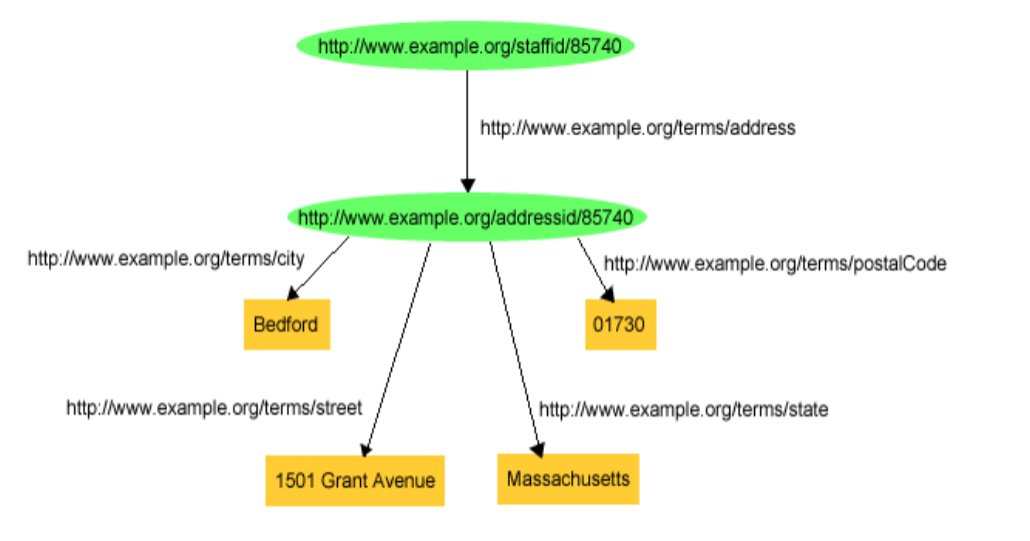
\includegraphics[width=0.7\textwidth]{_files/_images/rdf2.png}
    \caption{Rappresentazione a grafo, del codice turtle sopra}
    \label{fig:etichetta}
\end{figure}
\begin{warning}{Problema}
In questo modo però si generano numerosi URIref di servizio , come ad esempio
exaddressid:85740 per reificare informazioni aggregate. Tuttavia
dall'esterno nessuno può voler riferirsi direttamente a queste reificazioni per questo
non sembra che meritino degli identificatori universali come gli URIref
\end{warning}
Per questo motivo RDF consente di usare in questi casi dei blank node.
\begin{definition}{Blank Node}
    Un blank node è un nodo con una etichetta anonima (ovvero non associata a nessun URI).

    Un blank node viene rappresentato in RDF standard, in questo modo:
    \begin{center}
        \texttt{\_:identificativo}
    \end{center}
\end{definition}
L'identificativo del Blank Node (come \texttt{\_:b1} o \texttt{\_:node123}) è un puro artificio locale: ha valore soltanto all'interno di quel determinato documento o modello RDF.
\begin{itemize}
    \item  Non è un identificativo globale: Fuori da quel modello RDF specifico, l'ID del Blank Node non esiste. Non puoi usarlo come indirizzo sul Web.
    Invece l'URI è un identificativo globale.
    \item Non puoi fare un lookup diretto: Non potendo digitare una richiesta web diretta per quello specifico Blank Node, non puoi interrogarlo isolatamente per dire ``Web, dammi le informazioni sul nodo \texttt{\_:\allowbreak b1}.''
\end{itemize}
\textbf{Un blank node può occorrere come soggetto o oggetto di una tripla, non come
predicato}

Quindi questi sono i principali pezzi del RDF standard, le risorse, i blank node e i literal.
\section{Containers}
Il dizionario rdf, definisce alcuni tipi primitivi, detti container, per descrivere informazioni aggregate.
I container possono essere:
\begin{itemize}
    \item \textbf{Seq} : sequenza ordinata di nodi.
    \item \textbf{Bag} : collezione non ordinata di nodi.
    \item \textbf{Alt} :  lista di alternative equivalenti.
\end{itemize}
E' possibile avere ripetizioni, non vi è nessun meccanismo che forzi valori univoci.
RDF fornisce dei predicati built-in rdf:\_n per riferirsi ai vari componenti di container. Questi
predicati sono usati per istanziare indifferentemente Seq, Bag, o Alt ma chiaramente la
numerazione è significativa solo per le Seq.

\begin{figure}[htbp]
    \centering
    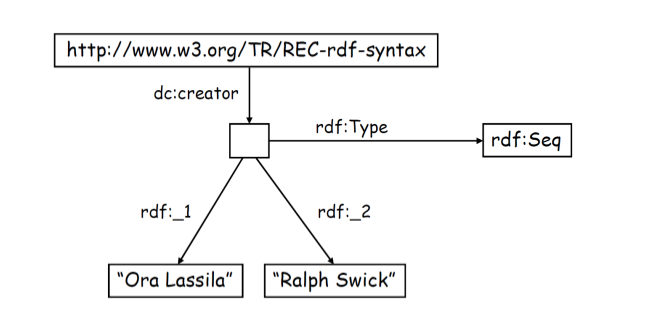
\includegraphics[width=0.7\textwidth]{_files/_images/rdf3.png}
    \caption{Esempio di Container}
    \label{fig:etichetta}
\end{figure}
\begin{lstlisting}
<http://www.w3.org/TR/REC-rdf-syntax> dc:creator _:seq.
_:seq rdf:Type rdf:Seq.
_:seq rdf:_1 "Ora Lassila".
_:seq rdf:_2 "Ralph Swick".
\end{lstlisting}
Qui tramite il dizionario rdf, stiamo definendo un container, dove gli elementi (in questo caso ordinati) sono quelle due stringhe.
\newpage

\section{Reificazione}
La reificazione è il meccanismo on cui in RDF è possibile prendere un'intera tripla (un statement) e trasformarla in una risorsa del grafo.
RDF fornisce dei predicati built-in per la reificazione:
\begin{itemize}
    \item \textbf{rdf:statement} : La classe che definisce che una determinata risorsa è una tripla reificata.   
    \item \textbf{rdf:subject} : Il predicato che indica qual è il soggetto della tripla originale.
    \item \textbf{rdf:predicate} : Il predicato che indica qual è il predicato della tripla originale.
    \item \textbf{rdf:object} : Il predicato che indica qual è l'oggetto della tripla originale.
\end{itemize}
\begin{figure}[htbp]
    \centering
    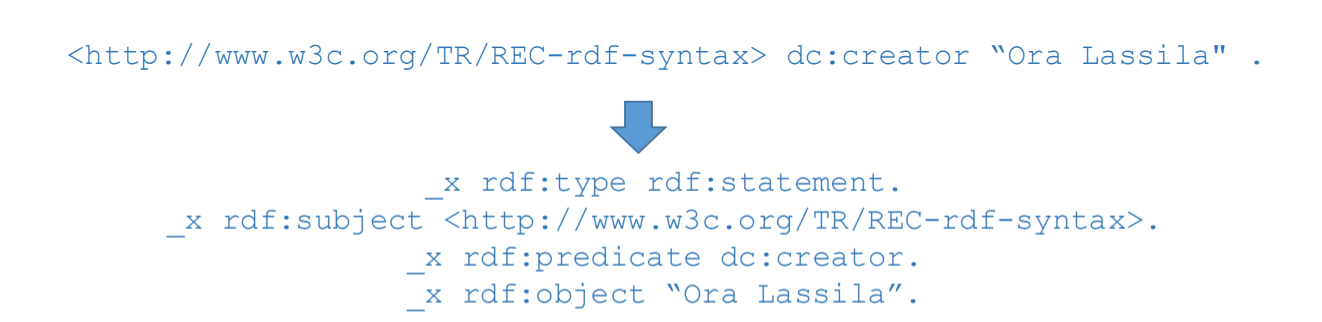
\includegraphics[width=0.7\textwidth]{_files/_images/rdf4.png}
    \caption{Esempio di reificazione dello statement}
    \label{fig:etichetta}
\end{figure}
\textbf{Ora lo statement è identificato dal blank node \_x}, ed è possibile esprimere il fatto che la Digital Library ha scritto questo statement
\begin{center}
    \_x dc:creator ``Digital Library''.
\end{center}


\end{document}
